%%%%%%%%%%%%%%%%%%%%%%%%%%%%%%%%%%%%%%%%%
% Journal Article
% LaTeX Template
% Version 1.3 (9/9/13)
%
% This template has been downloaded from:
% http://www.LaTeXTemplates.com
%
% Original author:
% Frits Wenneker (http://www.howtotex.com)
%
% License:
% CC BY-NC-SA 3.0 (http://creativecommons.org/licenses/by-nc-sa/3.0/)
%
%%%%%%%%%%%%%%%%%%%%%%%%%%%%%%%%%%%%%%%%%

%----------------------------------------------------------------------------------------
%	PACKAGES AND OTHER DOCUMENT CONFIGURATIONS
%----------------------------------------------------------------------------------------

\documentclass[twoside]{article}

\usepackage{lipsum} % Package to generate dummy text throughout this template
%\usepackage[showframe]{geometry}% http://ctan.org/pkg/geometry

\usepackage[sc]{mathpazo} % Use the Palatino font
\usepackage[T1]{fontenc} % Use 8-bit encoding that has 256 glyphs
\linespread{1.05} % Line spacing - Palatino needs more space between lines
\usepackage{microtype} % Slightly tweak font spacing for aesthetics
\usepackage{graphicx}
\usepackage[hmarginratio=1:1,top=32mm,columnsep=20pt]{geometry} % Document margins
\usepackage{multicol} % Used for the two-column layout of the document
\usepackage[hang, small,labelfont=bf,up,textfont=it,up]{caption} % Custom captions under/above floats in tables or figures
\usepackage{booktabs} % Horizontal rules in tables
\usepackage{float} % Required for tables and figures in the multi-column environment - they need to be placed in specific locations with the [H] (e.g. \begin{table}[H])
\usepackage{hyperref} % For hyperlinks in the PDF
\usepackage{amsmath}
\usepackage{lettrine} % The lettrine is the first enlarged letter at the beginning of the text
\usepackage{paralist} % Used for the compactitem environment which makes bullet points with less space between them
\usepackage{authblk}

\usepackage{abstract} % Allows abstract customization
\renewcommand{\abstractnamefont}{\normalfont\bfseries} % Set the "Abstract" text to bold
\renewcommand{\abstracttextfont}{\normalfont\small\itshape} % Set the abstract itself to small italic text
%\usepackage{apacite}
\bibliographystyle{ieeetr}

\usepackage{titlesec} % Allows customization of titles
\renewcommand\thesection{\Roman{section}} % Roman numerals for the sections
\renewcommand\thesubsection{\Roman{subsection}} % Roman numerals for subsections
\titleformat{\section}[block]{\large\scshape\centering}{\thesection.}{1em}{} % Change the look of the section titles
\titleformat{\subsection}[block]{\large}{\thesubsection.}{1em}{} % Change the look of the section titles

\usepackage{fancyhdr} % Headers and footers
\pagestyle{fancy} % All pages have headers and footers
\fancyhead{} % Blank out the default header
\fancyfoot{} % Blank out the default footer
\fancyhead[C]{}
%Running title $\bullet$ November 2012 $\bullet$ Vol. XXI, No. 1} % Custom header text
\fancyfoot[RO,LE]{\thepage} % Custom footer text

%----------------------------------------------------------------------------------------
%	TITLE SECTION
%----------------------------------------------------------------------------------------

\title{\vspace{-15mm}\fontsize{24pt}{10pt}\selectfont\textbf{BioJS-HGV Viewer: Genetic Variation Visualizer}} % Article title

%\author{
%\large
%\textsc{Saket K Choudhary}\thanks{Molecular and Computational Biology, University of Southern California, Los Angeles, California, USA}\\[2mm] % Your name
%\textsc{Leyla J Garcia}\thanks{European Bioinformatics Institute EMBL-EBI, Hinxton, Cambridge, CB10 1SD, UK} \textsc{Andrew Nightingale}\thanks{European Bioinformatics Institute EMBL-EBI, Hinxton, Cambridge, CB10 1SD, UK}\\[2mm] % Your name
%%\normalsize University of California \\ % Your institution
%\normalsize \href{mailto:skchoudh@usc.edu}{skchoudh@usc.edu} % Your email address
%\vspace{-5mm}
%}

\author[1]{Saket Choudhary\thanks{skchoudh@usc.edu}} %\thanks{Molecular and Computational Biology, University of Southern California}}
\author[2]{Leyla Garcia} %\thanks{European Bioinformatics Institute EMBL-EBI, Hinxton, Cambridge, CB10 1SD, UK}}
\author[2]{Andrew Nightingale} %\thanks{European Bioinformatics Institute EMBL-EBI, Hinxton, Cambridge, CB10 1SD, UK}}

\affil[1]{Molecular and Computational Biology, University of Southern California, Los Angeles, USA} %Department of Computer Science, \LaTeX\ University}
\affil[2]{European Bioinformatics Institute EMBL-EBI, Cambridge, England} %Department of Mechanical Engineering, \LaTeX\ University}
\date{}

%----------------------------------------------------------------------------------------

\begin{document}

\maketitle % Insert title

\thispagestyle{fancy} % All pages have headers and footers

%----------------------------------------------------------------------------------------
%	ABSTRACT
%----------------------------------------------------------------------------------------

\begin{abstract}

\noindent % \lipsum[1] % Dummy abstract text

Genomic studies have resulted in  catalogs of genetic variants in humans. Studying the pattern of damaging and non-damaging variants can not only help understand evolution but can also potentially improve human health by identifying the key driver elements.

We present BioJS-HGV Viewer, a BioJS component to represent and visualize genetic variants pooled from various sources. The component presents information at different levels allowing the end user to study the pattern of variations in detail in a user friendly manner. 

The code for BioJS-HGV Viewer is available at:\\ \url{https://github.com/saketkc/biojs-genetic-variation-viewer}.

A demo is available at: \url{http://saketkc.github.io/biojs}

\end{abstract}

%----------------------------------------------------------------------------------------
%	ARTICLE CONTENTS
%----------------------------------------------------------------------------------------

\begin{multicols}{2} % Two-column layout throughout the main article text

\section{Introduction}

\lettrine[nindent=0em,lines=3]{W} 
%orem ipsum dolor sit amet, consectetur adipiscing elit.
%\lipsum[2-3] % Dummy text
ith the advent of next-generation sequencing technologies, it has been possible to profile genomes in large numbers. One of the chief outcomes of such projects has been catalog of genetic variants such as dbSNP\cite{Smigielski2000} and COSMIC\cite{Forbes2011}. These catalogs contain publicly accessible sets of genetic variants found in humans which can be utilized to  study evolutionary relationships and disease specific variations. COSMIC database is a curated set of somatic mutations as observed in cancer samples. The number of such variations are   huge. dbSNP 129 had reportedly more than 14 million unique variants \cite{ncbiweb}. The availability of data at such a large scale makes the analysis challenging.

Any exploratory attempt at making sense of the variation data would involve visualizing the variants across the genome to determine specific sites, if any where the mutations are more frequent or are absent completely. 
 BioJS-HGV Viewer is a BioJS \cite{Corpas2014} component developed to visualize genetic variants in a comprehensive manner.BioJS is an open source project providing various components to visualize biological data. These components use javascript for rendering visualization. The visualizations are web based and hence are absolutely platform independent.
 
 
%------------------------------------------------

\section{Methods}
The functionality provided by BioJS-HGV Viewer has two parts:\\
\begin{compactitem}
\item Overview
\item Detailed or Zoomed View
\end{compactitem}
The architecture of this component is designed to handle both DNA and protein variants. The current implementation makes use of protein variants. These variant sites have been generated by an un-published webservice made available through EBI. This service has an indexed database of protein variants as reported in the COSMIC and UniProt\cite{Wu2006} database and is made available as a JSON\cite{json} file. The support for standard data formats such as VCF\cite{vcf} is under process.

By default  SIFT and Polyphen scores are averaged and the type of mutations are then decided based on this average score. The component however allows user to choose from either or all of the scores.

The demo at \url{http://saketkc.github.io/biojs} loads the protein \textit{J3KP33}. The component however allows loading other proteins by passing an additional argument to the url. For example: \url{http://saketkc.github.io/biojs/src/test/javascript/TestHGVViewer.html?q=P00533}

The user can also choose to hide a particular category of mutations. Both the overview and detailed mode have another \textit{'open view'}\ref{openview} where these mutations can further be separately visualized as \textit{Stop Gained}, \textit{Missense} and \textit{Splice Region}.


\subsection{Overview Mode}
In the default mode the viewer presents variant information in a condensed format focusing on the number and \textit{type of mutations} at each site. The type of mutations are classified as:
\begin{compactitem}
\item \textbf{Benign} %: Mutations that do not metastasize  and are virtually harmless 
\item \textbf{Damaging} %: Mutations that lead to 
\item \textbf{Mixed}
\end{compactitem}

The 'Mixed' category represents an \textbf{intermediate} state between damaging and benign.


The classification currently uses the predictions scores of Polyphen\cite{Ramensky2002} and SIFT\cite{Kumar2009}. Polyphen generate scores on a scale of $[0,1]$ with $1$ indicating that the mutation is damaging and $0$ indicating the mutation being benign. SIFT scores also operate on the scale of $[0,1]$ however $0$ indicates a damaging mutation.
The webservice has a database of all mutations with pre-generated scores for mutations across all proteins which can be retrieved as a JSON file.

The data thus received is parsed for calculating the number of mutations in each category. Each category is defined by threshold levels. For example a Polyphen score between 0.75 and 1.0 can be considered to reflect a damaging mutation. These threshold levels can be modified by the user.

%By default, the SIFT and Polyphen scores are averaged to generate a combined prediction score. 

\subsection{Detailed View}
In the detailed view\ref{zoomedtooltip} each individual amino acid on the protein is displayed as a rectangular box with all variants at that site. The box for variants is colored based on its type. On a \textit{mouse over} action at the variant box, the tooltip shows detailed information about that particular mutation.





%\begin{figure*}
%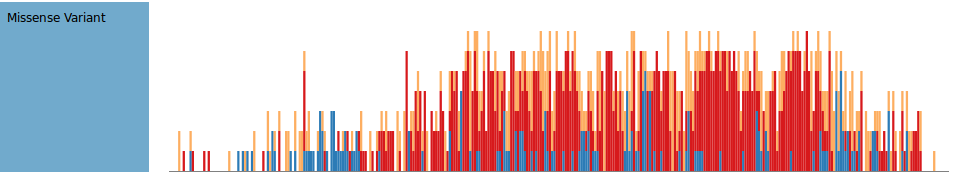
\includegraphics[width=\linewidth]{openview0}
%\caption{'Overview' of genetic variants as shown in by HGV viewer}
%\end{figure*}

%\begin{figure*}
%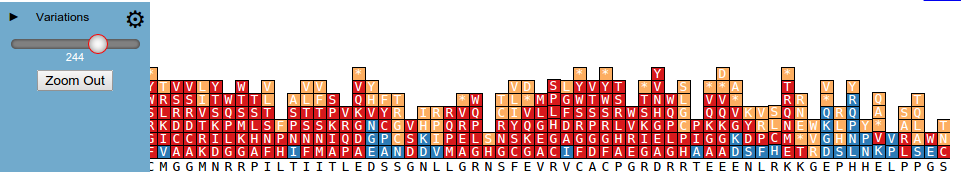
\includegraphics[width=\linewidth]{zoomed0}
%\caption{'Detailed view' of genetic variants. The SIFT/Polyphen scores and associated information with the mutations is rendered using tooltips(not shown here)}
%\end{figure*}





%------------------------------------------------

%\section{Results}

%\begin{table}[H]
%\caption{Example table}
%\centering
%\begin{tabular}{llr}
%\toprule
%\multicolumn{2}{c}{Name} \\
%\cmidrule(r){1-2}
%First name & Last Name & Grade \\
%\midrule
%John & Doe & $7.5$ \\
%Richard & Miles & $2$ \\
%\bottomrule
%\end{tabular}
%\end{table}


%------------------------------------------------

\section{Discussion}

BioJS-HGV Viewer can be used to study the pattern of mutations. A visual inspection can help discover sites of conserved regions or regions which are frequently mutated. 
Being entirely web based, it can be accessed from any platform.


%----------------------------------------------------------------------------------------
%	REFERENCE LIST
%----------------------------------------------------------------------------------------


\section{Acknowledgments}
We would like to thank the BioJS community for insightful discussions. This project was funded by Google Summer of Code 2014.

\bibliography{biojs_paper}


%----------------------------------------------------------------------------------------
\begin{figure*}
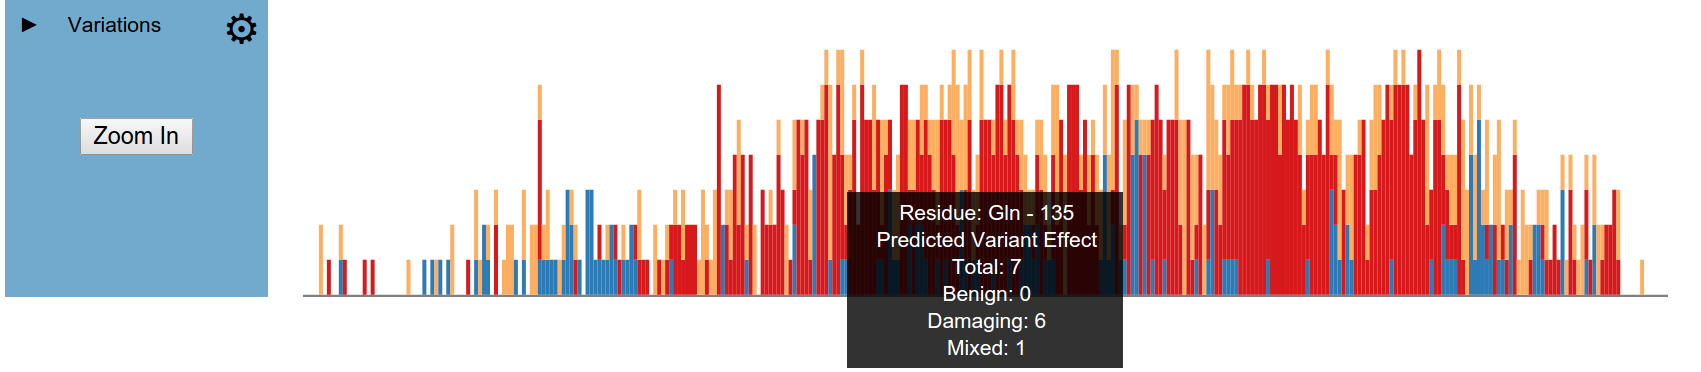
\includegraphics[width=\linewidth]{images/overview_withtooltip}
\label{overviewtooltip}
\caption{'Overview' of genetic variants as shown in by HGV viewer. Tooltips are used to display the number of mutations in benign, damaging and mixed categories.}
\end{figure*}
\begin{figure*}

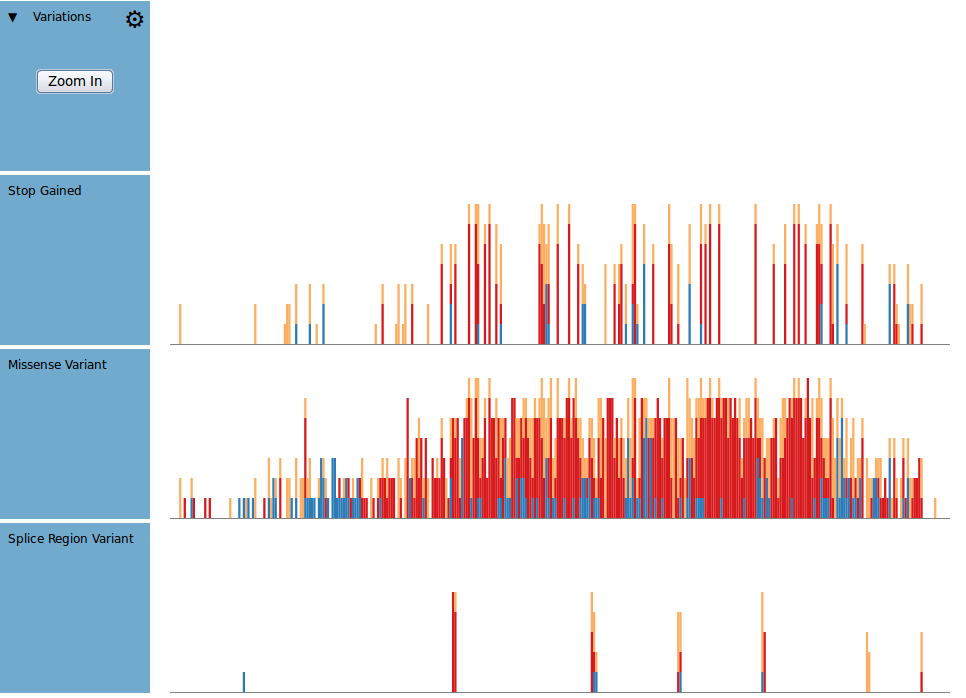
\includegraphics[width=\linewidth]{images/openview}
\caption{Overview with \textit{open view} ON}
\label{openview}
\end{figure*}

\begin{figure*}
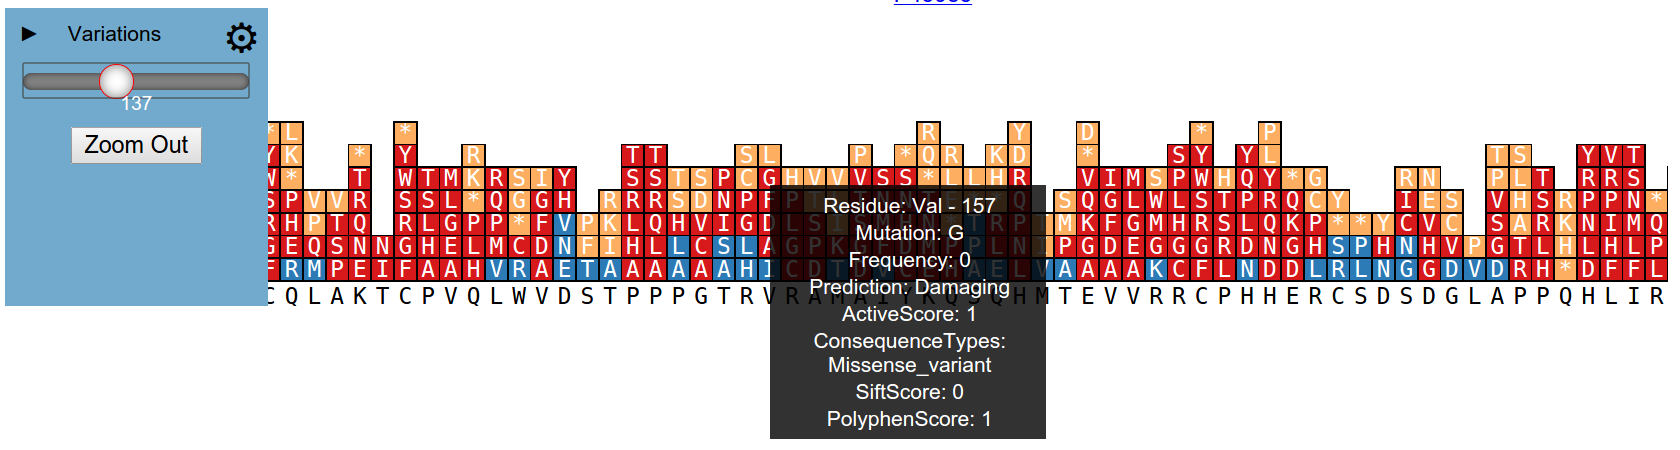
\includegraphics[width=\linewidth]{images/zoomed_withtooltip}
\caption{'Detailed view' of genetic variants. The SIFT/Polyphen scores and associated information with the mutations is rendered using tooltips}
\label{zoomedtooltip}
\end{figure*}

\begin{figure*}
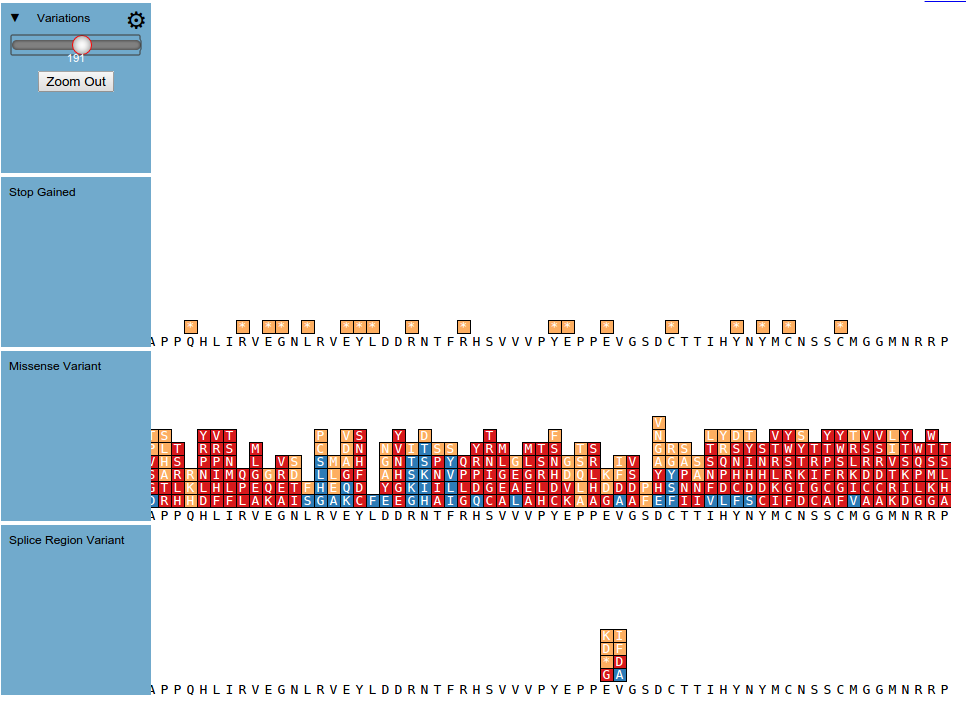
\includegraphics[width=\linewidth]{images/zoomedopen}
\caption{Zoomed with  open view}
\label{openwithzoomed}
\end{figure*}


\end{multicols}

\end{document}